\documentclass[aspectratio=169]{beamer}
\usetheme{TPU}
% Моя преамбула

% Математические формулы
\usepackage{amsmath}%,amssymb,amsfonts,pxfonts}
\usepackage{unicode-math}

% Переносы слов
\usepackage{polyglossia}
\setmainlanguage{russian}
\setotherlanguage{english}
\sloppy
\PolyglossiaSetup{russian}{indentfirst=true}

% Форматирование текста и математических формул
%\setmainfont{XITS}
%\setmathfont{XITS Math}

\setmainfont
[    Extension = .otf,
   UprightFont = *-regular,
      BoldFont = *-bold,
    ItalicFont = *-italic,
BoldItalicFont = *-bolditalic,
]{xits}

\setmathfont
[    Extension = .otf,
      BoldFont = *bold,
]{xits-math}

\usepackage[Symbol]{upgreek}

% Жирный курсив
\newcommand{\boldit}[1]{\textbf{\textit{#1}}}
% Мануальная нумерация
\usepackage{enumerate}

% Секции по центру
\usepackage{titlesec}
\titleformat*{\section}{\centering\normalfont\large\bfseries}
% \titleformat*{\subsection}{\normalfont\normalsize\bfseries}
\titleformat{\subsection}[block]{\hspace{\parindent}\bfseries}{\thesubsection}{0.2cm}{}
% Секции без нумерации
\newcommand{\anonsection}[1]{\section*{#1}\addcontentsline{toc}{section}{#1}}
% Нумерация картинок и таблиц
\usepackage{chngcntr}
\counterwithin{figure}{section}
\counterwithin{table}{section}

% Картинки
\usepackage[final]{graphicx}
\graphicspath{{../results/}} % images folder
% Вставить картинку
\newcommand{\imgh}[5][h]
{
    \begin{figure}[#1]
    \centering
    \includegraphics[#3]{#2}
    \caption{#4}
    \label{ris:#5}
    \end{figure}
}
%example: \imgh{1.pdf}{width=0.93\textwidth}{Image}{img}
\RequirePackage{caption}
\DeclareCaptionLabelSeparator{dot}{. }
\captionsetup{justification=centering,labelsep=dot}

% Поля страницы
\usepackage[left=2cm,right=2cm,top=2.5cm,bottom=2.5cm]{geometry}

% Полуторный интервал
\linespread{1.3}
% Нумерация страниц
\usepackage{fancyhdr}
\pagestyle{fancy}
\fancyhead{} % No page header
\fancyfoot[L]{} % Empty
\fancyfoot[C]{} % Empty
\fancyfoot[R]{\thepage} % Remove headlines
% Remove header underlines
\renewcommand{\headrulewidth}{0pt}

% Таблицы
\usepackage{multirow}
\usepackage{tabularx}
\newcolumntype{Y}{>{\centering\arraybackslash}X}
\newcolumntype{R}{>{\raggedleft\arraybackslash}X}
\renewcommand{\tabularxcolumn}[1]{>{\normalsize}b{#1}}
% Подгон больших таблиц под размер страницы
\usepackage{adjustbox}
\usepackage{bigstrut}
\usepackage{color,colortbl}
\definecolor{Gray}{gray}{0.9}

\renewcommand{\abstractname}{Аннотация}
\bibliographystyle{abbrv}

% Пакет для алгоритмов
\usepackage{algorithm}
\usepackage{algpseudocode}
\renewcommand{\algorithmicrequire}{\textbf{Вход:}}
\renewcommand{\algorithmicensure}{\textbf{Выход:}}
\floatname{algorithm}{Алгоритм}

\title{Копулярные модели для оценивания инвестиционного риска}
\author[Смагулов Д., Семёнов М.\,Е.]{%
  \texorpdfstring{%
    \begin{columns}
      \column{.5\linewidth}
      \raggedleft
      Смагулов Даулет \\ студент гр. 0ВМ61 ОЭФ ИЯТШ
      \column{.5\linewidth}
      \raggedright
      Семёнов Михаил Евгеньевич \\ к.\,ф.-м.\,н., доцент ОЭФ ИЯТШ
    \end{columns}
 }{Смагулов Даулет, Семёнов Михаил}
}
\institute{Томкий политхенический университет}
\date{\today}

\begin{document}

\titlepage

% Uncomment these lines for an automatically generated outline.
%\begin{frame}{Outline}
%  \tableofcontents
%\end{frame}

\section{Цели и задачи}

\begin{frame}{\insertsection}
    \textbf{Цель работы:} построить систему оценивания риска с использованием копулярных моделей.
    \vskip 2ex
    \textbf{Задачи:}
    \begin{itemize}
        \item проанализовать сущестующие подходы и выбрать метод для оценки параметров копулярных моделей.
        \item с использованием копулярных моделей вычислить и сравнить поведение различных мер риска (VaR, CVaR) для инвестиционного портфеля.
    \end{itemize}
\end{frame}

\section{Введение}
\subsection{Что такое копула}

\begin{frame}
    \frametitle{\insertsection}
    \framesubtitle{\insertsubsection}
    \begin{columns}
        \column{.5\linewidth}
        \begin{block}{Определение}
            \textbf{Копула} -- многомерная функция распределения, обладающая следующими свойствами: 
            \begin{itemize}
                \item область определения -- единичный гиперкуб размерности $d$ -- $[0, 1]^d$;
                \item маргинальные (частные) распределения равномерны на отрезке $[0, 1]$.
            \end{itemize}
        \end{block}
        \column{.5\linewidth}
            \begin{figure}
                \centering \includegraphics[height=0.5\paperheight]{Copula-example.pdf}
                \caption{Гауссова копула доходностей RTS и SBRF}
                \label{fig:copulaExample}
            \end{figure}
    \end{columns}
\end{frame}

\subsection{Теорема Шкляра}

\begin{frame}{\insertsection}
    \framesubtitle{\insertsubsection}
    \cite{Sklar1959} \\
    Для произвольной $d$-мерной функции распределения $F(x_1,\ldots,x_d)$ с одномерными маргинальными функциями распределения $F_1(x_1), \ldots, F_d(x_d)$ существует копула $C$, такая что
    $$F(x_1,\ldots,x_d) = C(F_1(x_1), \ldots, F_d(x_d)).$$
    \pause
    Таким образом, понятие \textit{копулы} позволяет нам рассматривать информацию о маргинальных распределениях и зависимости между переменными отдельно друг от друга.
\end{frame}

\section{Методология}
\subsection{Подготовка данных}

\begin{frame}{\insertsection}
    \framesubtitle{\insertsubsection}
    Цены активов преобзовываются в логарифмические доходности:
    \begin{equation}
        r_{t,i}=\log \frac{p_{t,i}}{p_{t-1,i}},
    \end{equation}
    где
    \begin{itemize}
        \item $i \in \overline{1, d}$, $d$ -- число активов;
        \item $p_{t, i}$ -- цена $i$-го актива на момент $t$, $t\in \overline{1, T}$.
    \end{itemize}
\end{frame}

\begin{frame}{\insertsection}
    \framesubtitle{\insertsubsection}
    Коэффициент ранговой корреляции Кендалла \cite{Kendall1970}:
    \begin{equation}
        \tau = r \big( \text{sgn} (X_a - X_b), \text{sgn} (Y_a - Y_b) \big),
    \end{equation}
    где
    \begin{itemize}
        \item $(X_a, X_b)$ и $(Y_a, Y_b)$ -- независимые пары некоторых случайных величин $X$ и $Y$;
        \item $r(x, y)$ -- линейная корреляция Пирсона.
    \end{itemize}
\end{frame}

\subsection{Маргинальные распределения}

\begin{frame}{\insertsection}
    \framesubtitle{\insertsubsection}
    Чтобы отразить такие свойства финансовых временных рядов, как \textit{тяжёлые хвосты} или \textit{асимметрия}, для описания лог-доходностей были выбраны следующие маргинальные распределения:
    \begin{itemize}
        \item<2-> гиперболическое;
        \item<3-> устойчивое;
        \item<4-> Мейкснера.
    \end{itemize}
\end{frame}

\begin{frame}{\insertsection}
    \framesubtitle{\insertsubsection}
    \begin{block}{Гиперболическое распределение}
    Функция плотности гиперболического распределения \cite{Barndoff1983}:
    \begin{equation}
        f_H(x|\pi,\zeta,\delta,\mu) = \frac{1}{2 \sqrt{1+\pi^2} K_1(\zeta)} e^{-\zeta \left[ \sqrt{1+\pi^2} \sqrt{1 + \big( \frac{x - \mu}{\delta})^2} - \pi \frac{x - \mu}{\delta} \right]},
    \end{equation}
    где
    \begin{itemize}
        \item $K_1(x)$ -- модифицированная функция Бесселя третьего рода 1-го порядка~\cite{Bessel1824}, 
        \item $\pi \in \mathbb{R}$, $\zeta > 0$, $\delta > 0$, $\mu \in \mathbb{R}$.
    \end{itemize}
    \end{block}
\end{frame}

\begin{frame}{\insertsection}
    \framesubtitle{\insertsubsection}
    \begin{block}{Устойчивое распределение}
    Характеристическая функция устойчивого распределения~\cite{Nolan2009}:
    \begin{eqnarray}
        \varphi_S(x|\alpha,\beta,\gamma,\delta) &=& \exp{\left[ix\delta-|\gamma x|^\alpha \left(1 - i\beta\text{sgn}(x)\Phi(x)\right)\right]}, \\
        \Phi(x) &=& \left\{ \begin{aligned}
            & \left(|\gamma x|^{1-\alpha} - 1\right)\tan{\frac{\pi\alpha}{2}}, & & \alpha \ne 1, \\
            & -\frac{2}{\pi}\log{|\gamma x|}, & & \alpha = 1,
        \end{aligned} \right. \nonumber
    \end{eqnarray}
    где
    \begin{itemize}
        \item $\alpha \in (0;\ 2]$, $\beta \in [-1;\ 1]$, $\gamma > 0$, $\delta \in \mathbb{R}$, 
        \item $i$ -- мнимая единица.
    \end{itemize}
    \end{block}
\end{frame}

\begin{frame}{\insertsection}
    \framesubtitle{\insertsubsection}
    \begin{block}{Распределение Мейкснера}
    Функция плотности распределения Мейкснера \cite{Schoutens2002}:
    \begin{equation}
        f_M(x|\alpha,\beta,\delta,\mu) = \frac{ \left( 2 \cos{ \frac{\beta}{2}} \right)^{2 \delta}}{2 \alpha \pi \Gamma(2 \delta)} \exp{\frac{\beta(x - \mu)}{\alpha}} \left| \Gamma \left( \delta + i \frac{x - \mu}{\alpha} \right) \right|^2,
    \end{equation}
    где
    \begin{itemize}
        \item $\Gamma(z)$ -- гамма-функция с комплексным аргументом $z$, 
        \item $\alpha > 0$, $|\beta| < \pi$, $\delta > 0$, $\mu \in \mathbb{R}$.
    \end{itemize}
    \end{block}
\end{frame}

\begin{frame}{\insertsection}
    \framesubtitle{\insertsubsection}
    \begin{block}{Оценка параметров распределений (фитинг)}
        Оценка параметров гиперболического распределения была произведена методом Нелдера\,--\,Мида, устойчивого и Мейкснера -- методом дистанции Крамера\,--\,фон~Мизеса.
    \end{block}
    \begin{block}{Проверка качества фитинга распределений}
        Качество оценки было определено с помощтю тестов Колмогорова\,--\,Смирнова, Андерсона\,--\,Дарлинга и Крамера\,--\,фон~Мизеса.
    \end{block}
\end{frame}

\subsection{Копулярные функции}

\begin{frame}{\insertsection}
    \framesubtitle{\insertsubsection}
    \begin{block}{Эллиптические копулы}
        \begin{equation}
            C(u_1, u_2, \ldots, u_d | \theta) = F_d(F^{-1}(u_1 | \theta), F^{-1}(u_2 | \theta), \ldots, F^{-1}(u_d | \theta) | \theta),
        \end{equation}
        где
        \begin{itemize}
            \item $F(x)$ -- кумулятивная функция маргинального распределения, 
            \item $F^{-1}(p)$ -- обратная функция распределения, 
            \item $F_d(x_1, x_2, \dots, x_d)$ -- функция $d$-мерного совместного распределения, 
            \item $\theta$ -- вектор параметров.
        \end{itemize}
        В работе использовались такие виды эллиптических копул, как Гауссова и Стьюдента $t$.
    \end{block}
\end{frame}

\begin{frame}{\insertsection}
    \framesubtitle{\insertsubsection}
    \begin{block}{Архимедовы копулы}
        \begin{equation}
            C(u_1,u_2,\ldots,u_d|\theta) = \psi^{[-1]}(\psi(u_1|\theta)+\psi(u_2|\theta) + \ldots + \psi(u_d|\theta) | \theta ),
        \end{equation}
        где
        \begin{itemize}
            \item $\psi$: $[0,1] \rightarrow [0, \infty]$ -- непрерывная строго убывающая выпуклая функция такая, что $\psi(1) = 0$, также называемая \textit{функцией-генератором};
            \item $\psi^{[-1]}(p)$ -- псевдо-обратная функция, определяемая из уравнения:
            $$\psi^{[-1]}(p) = \left\{ \begin{aligned}
                & \psi^{-1}(p), & \ 0 \le p & \le \psi(0), \\
                & 0,            & \ \psi(0) \le p & \le \infty.
            \end{aligned} \right.$$
        \end{itemize}
        В данной работе использовались архимедовы копулы Клейтона, Гумбеля, Франка, а также независимая копула.
    \end{block}
\end{frame}

\begin{frame}{\insertsection}
    \framesubtitle{\insertsubsection}
    \begin{block}{Гауссова копула}
        \begin{equation}
            C_{Gauss}(u_1, u_2,\ldots, u_d|\rho) = \Phi \left( \Phi_1^{-1} (u_1), \Phi_2^{-1} (u_2), \ldots, \Phi_d^{-1} (u_d) | \Sigma \right),
        \end{equation}
        где
        \begin{itemize}
            \item $\Phi(x_1, x_2, \dots, x_d)$  -- кумулятивная функция $d$-мерного совместного Гауссового распределения,
            \item $\Phi_i^{-1}(p)$ -- обратная функция одномерного Гауссового распределения,
            \item $\Sigma$ -- корреляционная матрица.
        \end{itemize} 
    \end{block}
\end{frame}

\begin{frame}{\insertsection}
    \framesubtitle{\insertsubsection}
    \begin{block}{Копула $t$\,--\,Стьюдента}
        \begin{equation} \label{tCop}
            C_{t}(u_1, u_2,\ldots, u_d|\Sigma, \nu) = t \left( t_1^{-1} (u_1|\nu), t_2^{-1} (u_2|\nu), \ldots, t_d^{-1} (u_d|\nu) | \Sigma, \nu \right),
        \end{equation}
        где
        \begin{itemize}
            \item $t_d(x_1, x_2, \dots,x_d)$ -- кумулятивная функция $d$-мерного совместного $t$-распределения,
            \item $t^{-1}(p)$ -- обратная функция одномерного $t$-распределения,
            \item $\Sigma$ -- корреляционная матрица,
            \item $\nu \ge 2$ -- число степеней свободы.
        \end{itemize}
    \end{block}
\end{frame}

\begin{frame}{\insertsection}
    \framesubtitle{\insertsubsection}
    \begin{block}{Определение}
        Будем называть $d$-мерной \textit{иерархической копулой} функцию, построенную из $d(d - 1)/2$  двумерных (парных) копул~\cite{Bedfort2002}. 
        Структура этой функции определяется набором связанных деревьев $\mathcal{V} =\{T_1, T_2, \ldots, T_ {d-1}\}$ по следующим правилам:
        \begin{enumerate}[(1)]
            \item $T_1 = (V_1, E_1)$ -- дерево дерево с узлами $V_1 = \{1, 2, \ldots, d\}$ и ребрами $E_1$. 
            Это дерево является графом, в котором любые два узла связаны уникальной ветвью.
            \item Для $m = 2, 3,\ldots,d - 1$ дерево $T_m$ состоит из узлов $V_m = E_{m-1}$ и ребер $E_m$.
            \item Для $m = 2, 3,\ldots, d - 1$ два узла дерева $T_m$ могут быть связаны ребром только в случае, если соответствующие ребра дерева $T_{m-1}$ имеют общий узел~\cite{Czado2010}.
        \end{enumerate}
    \end{block}
\end{frame}

\begin{frame}{\insertsection}
    \framesubtitle{\insertsubsection}
    \begin{block}{Функция плотности иерархической копулы}
        Пусть $c_{j_e, k_e; D_e}$ -- двумерная (парная) копула для каждого ребра $e$ в некотором из $(d - 1)$ деревьев вайн-копулы~\cite{Czado2010}. 
        Обозначим через $j_e$ и $k_e$ индексы условных переменных $U_{j_e}$ и $U_{k_e}$. 
        Также обозначим через $D_e$ условную выборку, соответствующую ребру $e$. 
        Таким образом, $c_{j_e, k_e; D_e}$ -- копул-функция плотности распределения для двух случайных величин $U_{j_e|D_e}$ и $U_{k_e|D_e}$, где $U_{i|D} = C_{i|D} (U_i|U_D)$. 
        Окончательно, приведем функцию плотности для регулярной иерархической копулы в виде:
        \begin{equation}
            c(u_1, \ldots, u_d) = \prod_{m=1}^{d-1} \prod_{e \in E_m} c_{j_e,k_e;D_e} \left( C_{j_e|D_e} (u_{j_e}|\textbf{u}_{D_e}), C_{k_e|D_e} (u_{k_e}|\textbf{u}_{D_e}); \textbf{u}_{D_e} \right).
        \end{equation}
    \end{block}
\end{frame}

\begin{frame}{\insertsection}
    \framesubtitle{\insertsubsection}
    \begin{block}{Оценка параметров копул}
        Для оценки параметров копул необходимо исходный ряд лог-доходностей $\boldsymbol{r}_i = (r_{1,i}, \ldots, r_{T,i})^\intercal$ для всех исторических наблюдений каждого актива $i \in \overline{1,d}$ преобразовать в псевдо-наблюдения $\boldsymbol{u}_i$ по следующей формуле:
        \begin{equation}
            u_{t,i} = \frac{\text{rg}(r_{t,i})}{T + 1},\ \forall \ t \in \overline{1,T},\ i \in \overline{1,d},
        \end{equation}
        где
        \begin{itemize}
            \item $\text{rg}(r_{t,i})$ -- ранг $r_{t,i}$ (от наименьшего к наибольшему) по отношению к наблюдаемым значениям $r_{\tau,i}, \tau \in \overline{1,T}$.
        \end{itemize}
        По вычисленным псевдо-наблюдениям методом <<инверсии $\tau$ Кендалла>>~\cite{Koj2010} были оценены параметры копул.
    \end{block}
\end{frame}

\subsection{Оптимизация портфеля}

\begin{frame}{\insertsection}
    \framesubtitle{\insertsubsection}
    \begin{block}{Определение}
        Value-at-Risk (\textit{VaR}) -- минимальное значение потерь портфеля, которое не будет превышено с заданной вероятностью:
        \begin{equation}
            \textit{VaR}_\alpha = \min\left\{\zeta \in \mathbb{R}|P(\xi \le \zeta) \ge \alpha \right\},
        \end{equation}
        где
        \begin{itemize}
            \item $\zeta$ -- некоторое значение случайной величины $\xi$,
            \item $\mu_p$ -- ожидаемая доходность портфеля.
            \item $\alpha$ -- заданная вероятность, или уровень.
        \end{itemize}
    \end{block}
\end{frame}

\begin{frame}{\insertsection}
    \framesubtitle{\insertsubsection}
    \begin{block}{Определение}
        Conditional-Value-at-Risk (\textit{CVaR}) -- ожидаемое (среднее) значение потерь, которые не будут превышены с заданной вероятностью.
        \begin{equation}
            \textit{CVaR}_\alpha = \mathbb{E}\left\{-\mu_p | -\mu_p \ge VaR_\alpha \right\},
        \end{equation}
        где
        \begin{itemize}
            \item $\mu_p$ -- ожидаемая доходность портфеля.
            \item $\alpha$ -- заданная вероятность, или уровень.
        \end{itemize}
    \end{block}
\end{frame}

\begin{frame}{\insertsection}
    \framesubtitle{\insertsubsection}
    \begin{block}{Задача оптимизации}
        \begin{eqnarray}
            \underset{\textbf{w}}{\text{minimize}} & & \textit{CVaR}_\alpha \\
            \text{subject to} & & \sum_{i=1}^d \mu_i w_i \ge \bar{\mu}_p \nonumber \\
            & & \sum_{i=1}^d w_i = 1 \nonumber \\
            & & w_i \ge 0. \nonumber
        \end{eqnarray}
    \end{block}
\end{frame}

\subsection{Алгоритм вычисления мер риска}

\begin{frame}{\insertsection}
    \framesubtitle{\insertsubsection}
    \begin{block}{Вход}
        \begin{itemize}
            \item Лог-доходности $\{r_{i,t}\}$, $i \in \overline{1,d}$,
            \item весовые коэффициенты $w_i$ оптимального портфеля, 
            \item маргинальные распределения и параметры для каждого актива, 
            \item $d$-мерная копула с известными параметрами,
            \item уровень $\alpha$.
        \end{itemize}
    \end{block}
    \begin{block}{Выход}
        \begin{itemize}
            \item $\textit{VaR}_\alpha$ и $\textit{CVaR}_\alpha$.
        \end{itemize}
    \end{block}
\end{frame}

\begin{frame}{\insertsection}
    \framesubtitle{\insertsubsection}
    \begin{algorithm}[H]
    \scriptsize
    \caption{Расчёт риск-метрик с использованием копул}
    \label{Alg1}
    \begin{algorithmic}[1]
    	\Require Лог-доходности $\{r_{i,t}\}$, $i \in \overline{1,d}$, весовые коэффициенты $w_i$, маргиналы и их параметры, $d$-мерная копула и её параметры, уровень $\alpha$.
    	\State Сгенерировать массив псевдо-наблюдений 
    	$\{\hat{u}_{i,s}\} \in [0, 1]^d, \ i \in \overline{1,d}, \ s \in \overline{1, S}$ 
    	с помощью копулы.
    	\State Преобразовать сгенерированные псевдо-наблюдения в массив квантилей:
    	\For {$i \in \overline{1,d}$}
    	    \For {$s \in \overline{1,S}$}
    	        \State Присвоить $\hat{r}_{i,s} = F^{-1}_i (\hat{u}_{i,s})$.
    	    \EndFor
    	\EndFor
    	\State Вычислить ряд прибылей и потерь (P\&L) портфеля:
    	\For {$s \in \overline{1,S}$} 
    	\State Присвоить $\text{P\&L}(s) = \sum_{i=1}^d \hat{r}_{i,s} \cdot w_i$.
    	\EndFor
    	\State Вычислить $\textit{VaR}_\alpha$ и $\textit{CVaR}_\alpha$.
    	\Ensure VaR и CVaR для сгенерированных P\&L портфеля.
    \end{algorithmic}
    \end{algorithm}
\end{frame}

\begin{frame}{\insertsection}
    \framesubtitle{\insertsubsection}
    \begin{algorithm}[H]
    \footnotesize
    \caption{Бутстрап-процедура для оценки риск-метрик}
    \begin{algorithmic}[1]
    	\Require Число симуляций $N$, входные данные алгоритма~\ref{Alg1}.
    	\State Создать пустые векторы $\textit{VaR}_\alpha$ и $\textit{CVaR}_\alpha$.
    	\For {$i \in \overline{1,N}$}
    	    \State Запустить алгоритм~\ref{Alg1}
    	    \State Добавить полученные значения $\textit{VaR}_{\alpha, i}$ и $\textit{CVaR}_{\alpha, i}$ к векторам $\textit{VaR}_\alpha$ и $\textit{CVaR}_\alpha$ соответственно.
    	\EndFor
    	\State Вычислить средние значения векторов $\textit{VaR}_\alpha$ и $\textit{CVaR}_\alpha$.
    	\State Вычислить доверительный интервал векторов $\textit{VaR}_\alpha$ и $\textit{CVaR}_\alpha$.
    	\State Вычислить смещение, SD и RMSE векторов $\textit{VaR}_\alpha$ и $\textit{CVaR}_\alpha$.
    	\Ensure Средние значения, доверительный интервал, характеристики ошибок оценок VaR и CVaR.
    \end{algorithmic}
    \end{algorithm}
\end{frame}

\begin{frame}{\insertsection}
    \framesubtitle{\insertsubsection}
    Формулы для вычисления интервальных характеристик
    \begin{gather}
        \bar{x} = \mathbb{E} (\textbf{x}) \approx \frac{1}{N} \sum_{i=1}^N x_i, \hspace{0.5cm}
        \Delta = \bar{x} - \hat{x}, \label{boot-bias} \nonumber\\
        \text{SD} = \sqrt{\frac{1}{N-1} \sum_{i=1}^N (\bar{x} - x_i)^2}, \hspace{0.5cm}
        \text{RMSE} = \sqrt{\frac{1}{N-1} \sum_{i=1}^N (\hat{x} - x_i)^2}.\nonumber
    \end{gather}
    Формулы для вычисления доверительного интервала:
    \begin{equation}
        q^- = \mathbb{Q}_{\textbf{x}} (0.025), \ q^+ = \mathbb{Q}_{\textbf{x}} (0.975),\nonumber
    \end{equation}
\end{frame}

\section{Результаты расчётов}
\subsection{Исходные данные}

\begin{frame}{\insertsection}
    \framesubtitle{\insertsubsection}
    \begin{columns}
        \column{.5\linewidth}
        \begin{block}{Фьючерсы}
            \begin{itemize}
                \item индекс РТС (SPFB.RTS)
                \item ПАО {<<Газпром>>} (SPFB.GAZR)
                \item ПАО {<<Сбербанк>>} (SPFB.SBRF)
                \item ПАО ГМК {<<Норильский Никель>>} (SPFB.GMKR)
            \end{itemize}
        \end{block}
        \column{.5\linewidth}
        \begin{figure}
            \centering
            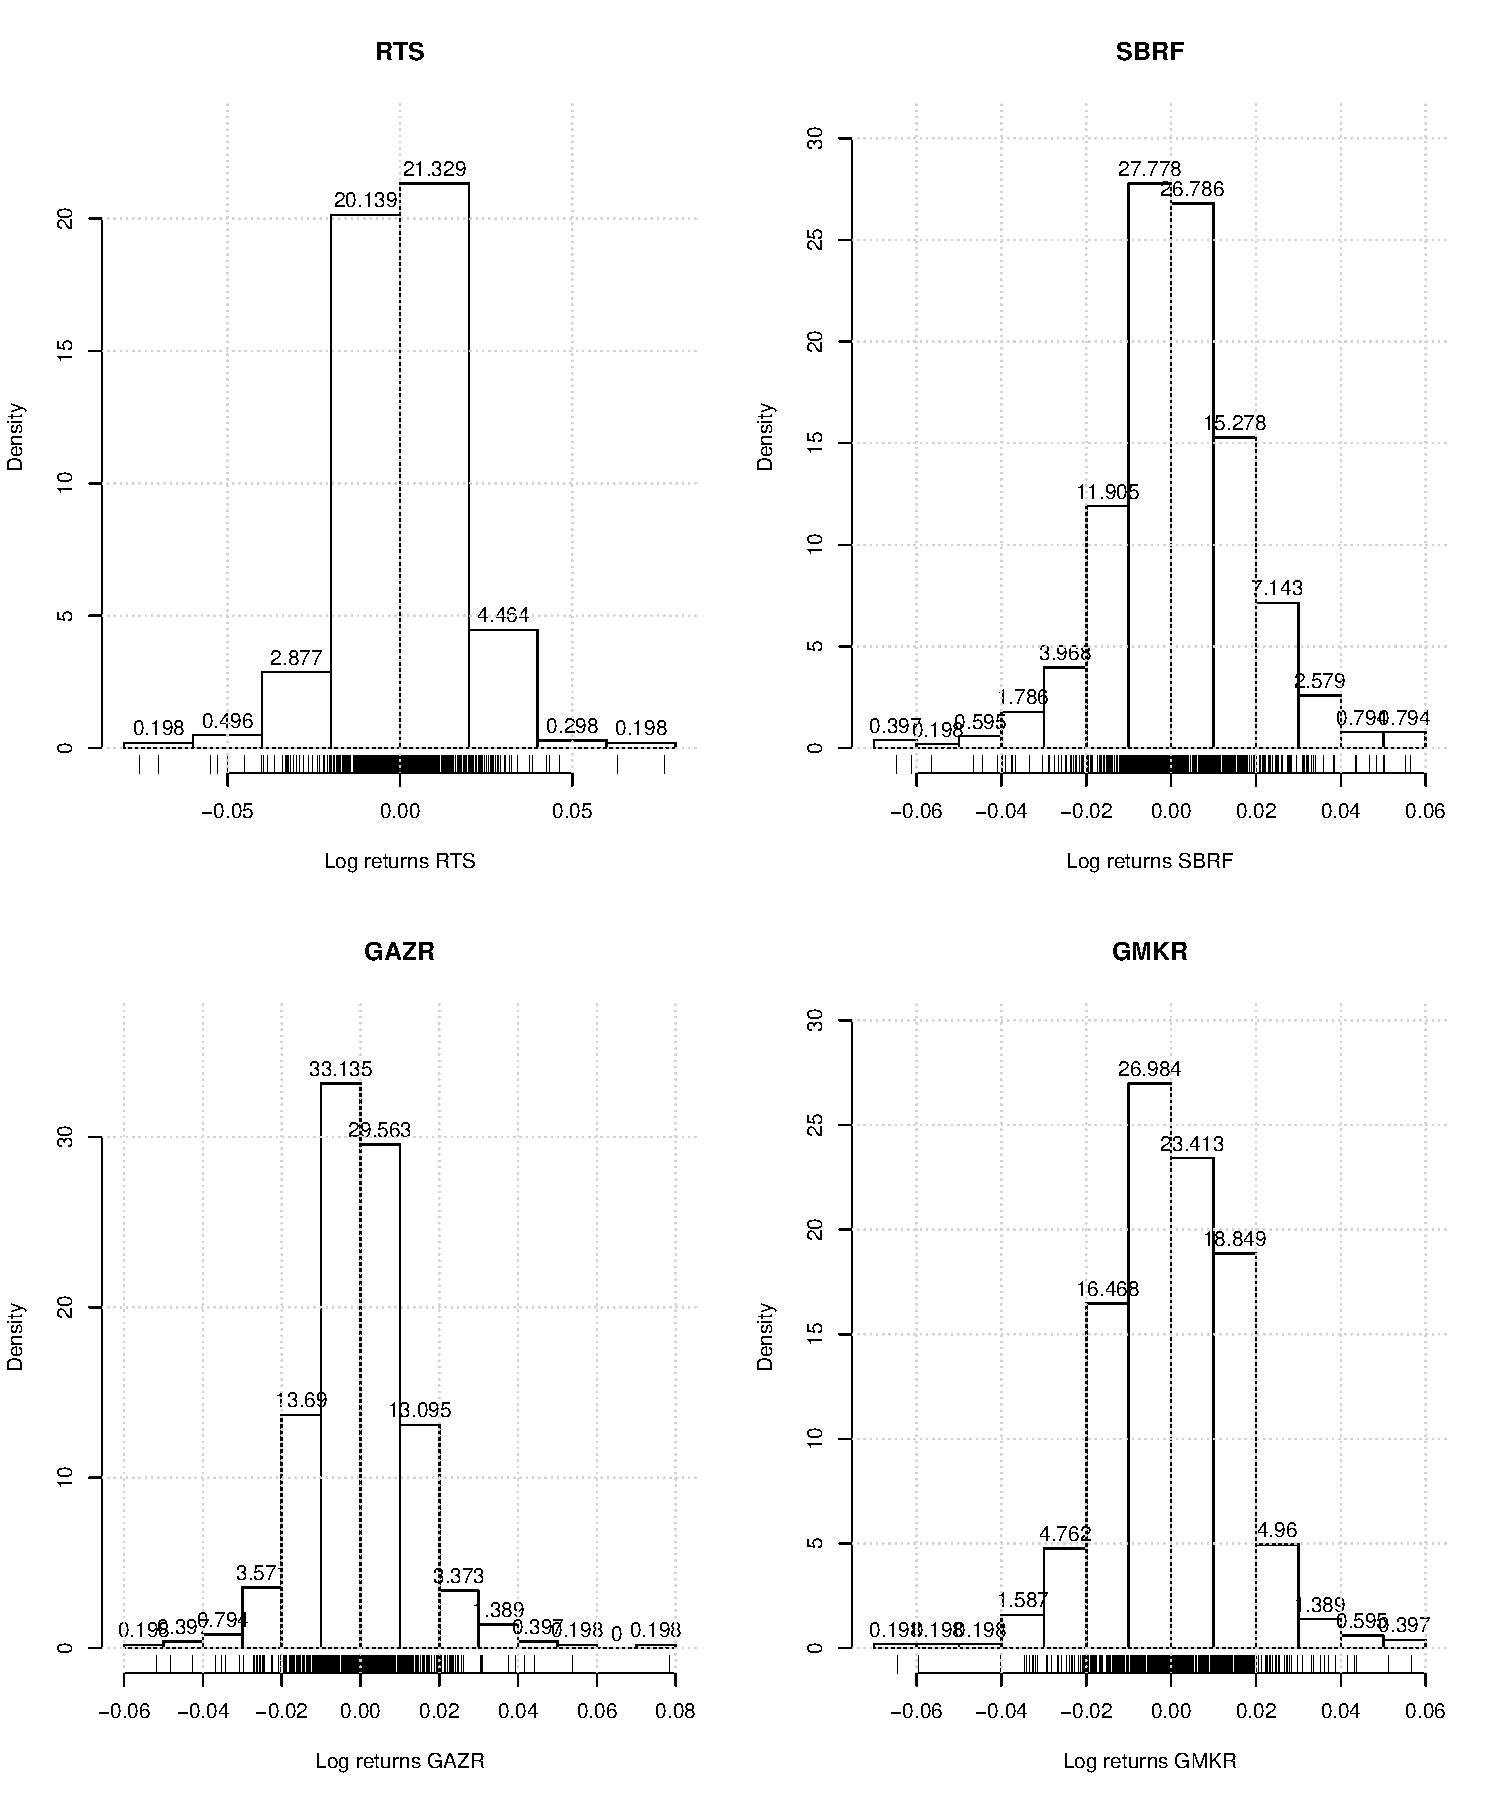
\includegraphics[height=0.6\paperheight]{Histogram.pdf}
            \caption{Гистограммы лог-доходностей активов}
        \end{figure}
    \end{columns}
\end{frame}

\begin{frame}{\insertsection}
    \framesubtitle{\insertsubsection}
    \begin{table}
        \centering
        \caption{Описательные  характеристики логарифмических доходностей}
        \begin{adjustbox}{max width=\textwidth}
        \begin{tabular}{l|cc|rrrr}
            \toprule
            \multirow{2}{*}{Активы} & \multicolumn{2}{c|}{Моменты} & \multicolumn{4}{c}{$\tau$ Кендалла} \\
            & $\mu$ & $\sigma$ & \multicolumn{1}{c}{RTS} & \multicolumn{1}{c}{SBRF} & \multicolumn{1}{c}{GAZR} & \multicolumn{1}{c}{GMKR} \\ 
            \midrule
    RTS  &  0.00075 & 0.016 &     1 & 0.515 & 0.444 & 0.218 \\
    SBRF &  0.00154 & 0.016 & 0.515 &     1 & 0.364 & 0.208 \\
    GAZR & -0.00001 & 0.013 & 0.444 & 0.364 &     1 & 0.256 \\
    GMKR &  0.00033 & 0.015 & 0.218 & 0.208 & 0.256 &     1 \\    
            \bottomrule
        \end{tabular}
        \end{adjustbox}
    \end{table}
\end{frame}

\subsection{Оценка параметров маргинальных распределений}

\begin{frame}{\insertsection}
    \framesubtitle{\insertsubsection}
    \begin{table}
        \centering
        \footnotesize
        \caption{Оценка параметров маргинальных распределений}
        \begin{tabularx}{\textwidth}
        {>{\hsize=2.4\hsize}X >{\hsize=0.4\hsize}Y *{4}{>{\hsize=0.8\hsize}R}}
        \hline 
        \multicolumn{2}{c}{Распределения и параметры} & \multicolumn{1}{r}{RTS} &
        \multicolumn{1}{r}{SBRF} & \multicolumn{1}{r}{GAZR} &
        \multicolumn{1}{r}{GMKR} \\ 
        \hline
        \multirow{4}{*}{\parbox{\hsize}{Гиперболическое\\ распределение}}
            &    $\pi$ &    0.00336 &    0.06100 &    0.06751 &    0.03301 \\
            &  $\zeta$ &    0.68417 &    0.80977 &    0.73310 &    3.31449 \\
            & $\delta$ &    0.00694	&    0.00823 &    0.00609 &    0.02232 \\
            &    $\mu$ &    0.00067 & $-$0.00003 & $-$0.00139 & $-$0.00076 \\ \hline
        \multirow{4}{*}{\parbox{\hsize}{Устойчивое распределение}}
            & $\alpha$ &    1.53561 &    1.56414 &    1.86326 &    1.92994 \\
            &  $\beta$ &    0.21114 &    0.22262 &    0.85066 &    0.66465 \\
            & $\gamma$ &    0.00884 &    0.00926 &    0.00770 &    0.00999 \\
            & $\delta$ &    0.00020 &    0.00063 & $-$0.00099 & $-$0.00016 \\ \hline
        \multirow{4}{*}{\parbox{\hsize}{Распределение Мейкснера}}
            & $\alpha$ &    0.03306 &    0.03064 &    0.02642 &    0.00428 \\
            &  $\beta$ &    0.30800 &    0.45599 &    0.22236 &    0.87412 \\
            & $\delta$ &    0.44168 &    0.51881 &    0.47397 &   18.31193 \\
            &    $\mu$ & $-$0.00099 & $-$0.00173 & $-$0.00143 & $-$0.03615 \\ \hline
        \end{tabularx}
    \end{table}
\end{frame}

\begin{frame}{\insertsection}
    \framesubtitle{\insertsubsection}
    \begin{table}
    \centering
    \caption{Значения $p$-value статистических тестов для распределений-кандидатов}
    \label{tab:margintest}
    \begin{tabularx}{\textwidth}
    {>{\hsize=1.6\hsize}X >{\hsize=1.6\hsize}X *{4}{>{\hsize=0.7\hsize}Y}}
    \toprule
    \multicolumn{1}{c}{Тест} & \multicolumn{1}{c}{Распределение} & RTS & SBRF & GAZR & GMKR \bigstrut \\ \midrule[1pt]
    \multirow{3}{*}{\parbox{\hsize}{Колмогорова\,--\,Смирнова}}
        & Гиперболическое & 0.91 & 0.88 & 1.00 & 0.79 \\
        & Устойчивое      & 0.89 & 0.94 & 0.87 & 0.94 \\
        & Мейкснера       & 0.99 & 0.95 & 1.00 & 0.96 \\ \midrule
    \multirow{3}{*}{\parbox{\hsize}{Андерсона\,--\,Дарлинга}}
        & Гиперболическое & 0.88 & 0.94 & 1.00 & 0.93 \\
        & Устойчивое      & 0.73 & 0.87 & 0.47 & 0.97 \\
        & Мейкснера       & 0.87 & 0.92 & 1.00 & 0.90 \\ \midrule
    \multirow{3}{*}{\parbox{\hsize}{Крамера\,--\,фон~Мизеса}}
        & Гиперболическое & 0.94 & 0.89 & 1.00 & 0.90 \\
        & Устойчивое      & 0.97 & 0.92 & 0.94 & 0.98 \\
        & Мейкснера       & 0.99\cellcolor{gray!33} & 0.95\cellcolor{gray!33} & 1.00\cellcolor{gray!33} & 0.98\cellcolor{gray!33} \\ \bottomrule
    \end{tabularx}
    \end{table}
\end{frame}

\subsection{Оценка параметров копул}

\begin{frame}{\insertsection}
    \framesubtitle{Получение псевдо-наблюдений}
    \begin{figure}
        \centering
        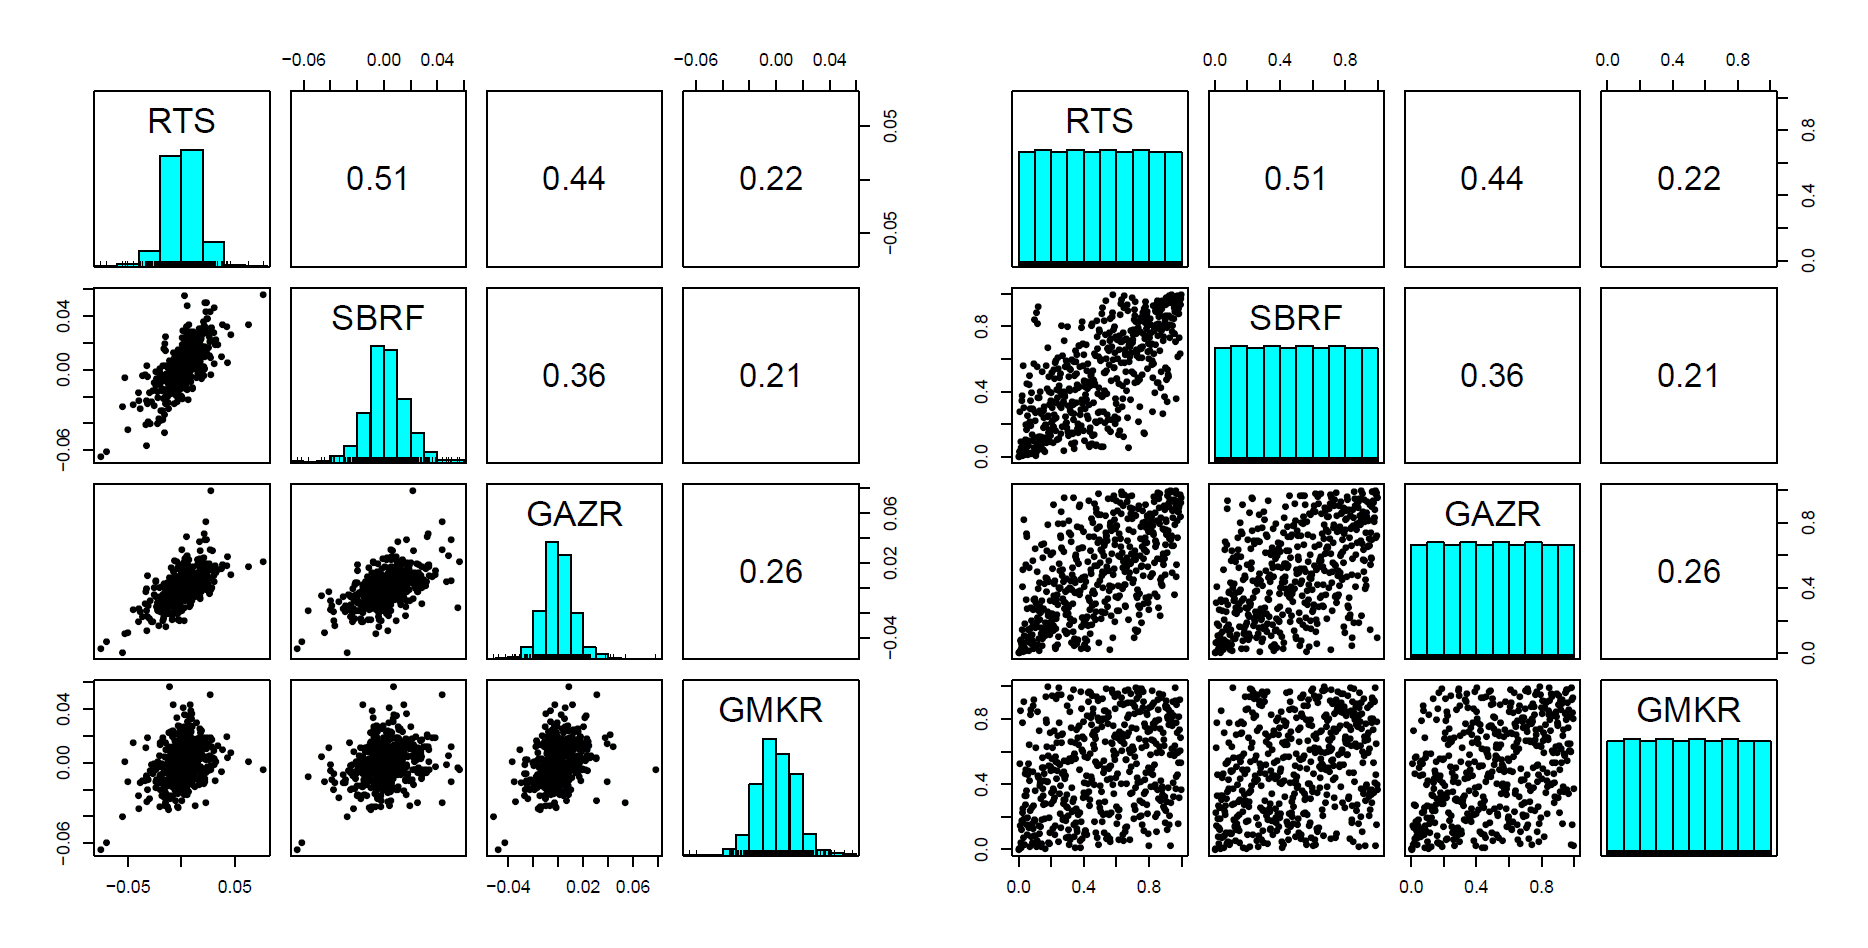
\includegraphics[height=0.6\paperheight]{pobs.png}
        \caption{Парные графики наблюдений (слева) и псевдо-наблюдений (справа)}
    \end{figure}
\end{frame}

\begin{frame}{\insertsection}
    \framesubtitle{\insertsubsection}
    \begin{block}{Гауссова копула}
    \begin{equation}
        \Sigma_{Gauss} = \left(
        \begin{array}{cccc}
            1 & & & \\
            0.723 & 1 & & \\
            0.642 & 0.540 & 1 & \\
            0.335 & 0.320 & 0.391 & 1
        \end{array} \right),
    \end{equation}
    \end{block}
    \begin{block}{$t$ копула}
    \begin{equation} \label{tcopfit}
        \Sigma_t = \left(
        \begin{array}{cccc}
            1 & & & \\
            0.723 & 1 & & \\
            0.642 & 0.540 & 1 & \\
            0.335 & 0.320 & 0.391 & 1
        \end{array} \right), \ \nu = 4.
    \end{equation}
    \end{block}
\end{frame}

\begin{frame}{\insertsection}
    \framesubtitle{\insertsubsection}
    \begin{block}{Иерархическая копула}
    \begin{enumerate}[(1)]
        \item Дерево 1:\\
        $c_{u_1;u_2}$ -- копула Стьюдента с параметрами $\rho=0.72$, $\nu=7.57$, $\tau=0.51$;\\
        $c_{u_3;u_1}$ -- копула Survival BB1 (повёрнутая на $180^{\circ}$ копула Клейтона-Гумбеля) с параметрами $\theta=0.12$, $\delta=1.68$, $\tau=0.44$;\\
        $c_{u_4;u_3}$ -- копула Survival Gumbel (повёрнутая на $180^{\circ}$ копула Гумбеля) с параметрами $\delta=1.33$, $\tau=0.25$;
        \item Дерево 2:\\
        $c_{u_3,u_2;u_1}$ -- копула Гумбеля с параметрами $\delta=1.1$, $\tau=0.09$;\\
        $c_{u_4,u_1;u_3}$ -- копула Клейтона с параметрами $\delta=0.16$, $\tau=0.07$;
        \item Дерево 3:\\
        $c_{u_4,u_2;u_3,u_1}$ -- копула Франка с параметрами $\delta=0.54$, $\tau=0.06$.
    \end{enumerate}
    \end{block}
\end{frame}

\begin{frame}{\insertsection}
    \framesubtitle{\insertsubsection}
    \begin{block}{Структура деревьев}
    \begin{figure}
        \centering
        \includegraphics[height=0.5\paperheight]{Trees.png}
        \caption{Парные графики наблюдений (слева) и псевдо-наблюдений (справа)}
    \end{figure}
    \end{block}
\end{frame}

\begin{frame}{\insertsection}
    \framesubtitle{\insertsubsection}
    \begin{table}
    \centering
    \caption{Значения статистичеческих критериев для выбранных копулярных моделей}
    \label{tab:coptest}
    \setlength{\tabcolsep}{8pt}
    \begin{tabular}{lrr}
    \toprule
    Копула & Статистика & $p$-value \\ \midrule
    Гауссова  & $S_n=0,034$ & 0,19 \\
    Стьюдента & $S_n=0,391$ & 0,05 \\
    R-vine    & $W=15,15$   & 0,95    \\ \bottomrule
    \end{tabular}
    \end{table}
\end{frame}

\subsection{Результаты оптимизации}

\begin{frame}{\insertsection}
    \framesubtitle{\insertsubsection}
    \begin{table}
        \caption{Сравнение риск-метрик равновесного и оптимального портфеля, полученных методом исторического моделирования} \label{tab:eqw-optim}
        \centering
        \setlength{\tabcolsep}{5pt}
        \begin{tabularx}{0.8\textwidth}
        {Y *{3}{R@{\ /\ }X}}
        \toprule
    \multirow{2}{*}{$\alpha$, \%} & \multicolumn{6}{c}{$\textit{VaR}_\alpha$ / $\textit{CVaR}_\alpha$, $\times 10^{-2}$} \\ \cmidrule{2-7} 
    & \multicolumn{2}{c}{Оптимальный} & \multicolumn{2}{c}{Равновесный} & \multicolumn{2}{c}{Смещение, $\times 10^{-2}$} \\ \midrule
    90.0 & $1.31$ & $2.01$ & $1.32$ & $2.14$ & $0.01$ & $0.13$ \\ 
    95.0 & $1.69$ & $2.48$ & $1.82$ & $2.74$ & $0.13$ & $0.25$ \\ 
    99.0 & $2.59$ & $3.96$ & $2.79$ & $4.36$ & $0.21$ & $0.41$ \\ 
    99.5 & $3.63$ & $5.22$ & $4.05$ & $5.50$ & $0.43$ & $0.28$ \\ 
    99.9 & $5.62$ & $5.86$ & $6.05$ & $6.29$ & $0.44$ & $0.43$ \\ 
    \bottomrule
        \end{tabularx}
    \end{table}
\end{frame}

\subsection{Расчёт точечных оценок риск-метрик}

\begin{frame}{\insertsection}
    \framesubtitle{\insertsubsection}
    \begin{table}
    \centering
    \caption{Значение эмпирической $\widehat{\textit{VaR}}$ и оценённой риск-метрики $\textit{VaR}^{est}$ c изпользованмием Гауссовой\,/\,Стьюдента\,/\,R-vine копул}
    \label{tab:var}
    \setlength{\tabcolsep}{5pt}
    \begin{adjustbox}{max width=\textwidth}
    \begin{tabularx}{\textwidth}{>{\hsize=0.8\hsize}Y|>{\hsize=1.2\hsize}Y 
    *{2}{|>{\setlength{\hsize}{0.4\hsize}}R
    *{2}{@{\,/\,}>{\setlength{\hsize}{0.4\hsize}}R}}}
    \toprule
    \multicolumn{1}{c|}{$\alpha$, \%} & \multicolumn{1}{c|}{$\widehat{\textit{VaR}}$, $\times 10^{-2}$} & \multicolumn{3}{c|}{$\textit{VaR}^{est}$, $\times 10^{-2}$} & \multicolumn{3}{c}{$\Delta$, $\times 10^{-3}$} \bigstrut[t] \\ \midrule
    90.0   & $1.31$ & $1.57$ & $1.71$ & $1.51$ & $2.55$ & $3.94$ & $1.94$ \\ 
    95.0   & $1.69$ & $2.15$ & $2.37$ & $1.94$ & $4.56$ & $6.81$ & $2.48$ \\ 
    99.0   & $2.59$ & $3.28$ & $3.64$ & $3.28$ & $6.95$ & $10.54$ & $6.97$ \\ 
    99.5 & $3.63$ & $3.70$ & $4.02$ & $3.94$ & $0.69$ & $3.95$ & $3.13$ \\ 
    99.9 & $5.62$ & $5.63$ & $5.83$ & $6.01$ & $0.12$ & $2.18$ & $3.90$ \\ \bottomrule
    \end{tabularx}
    \end{adjustbox}
    \end{table}
\end{frame}

\begin{frame}{\insertsection}
    \framesubtitle{\insertsubsection}
    \begin{table}
    \centering
    \caption{Значение  эмпирической $\widehat{\textit{CVaR}}$ и оценённой риск-метрики $\textit{CVaR}^{est}$ c изпользованмием Гауссовой\,/\,Стьюдента\,/\,R-vine копул}
    \label{tab:es}
    \setlength{\tabcolsep}{5pt}
    \begin{adjustbox}{max width=\textwidth}
    \begin{tabularx}{\textwidth}{>{\hsize=0.8\hsize}Y|>{\hsize=1.2\hsize}Y 
    *{2}{|>{\setlength{\hsize}{0.4\hsize}}R
    *{2}{@{\,/\,}>{\setlength{\hsize}{0.4\hsize}}R}}}
    \toprule 
    \multicolumn{1}{c|}{$\alpha$, \%} & \multicolumn{1}{c|}{$\widehat{\textit{CVaR}}$, $\times 10^{-2}$} & \multicolumn{3}{c|}{$\textit{CVaR}^{est}$, $\times 10^{-2}$} & \multicolumn{3}{c}{$\Delta$, $\times 10^{-3}$} \bigstrut[t] \\ \midrule
    90.0   & $2.01$ & $2.38$ & $2.58$ & $2.32$ & $3.68$ & $5.66$ & $3.12$ \\ 
    95.0   & $2.48$ & $2.95$ & $3.17$ & $2.92$ & $4.65$ & $6.89$ & $4.35$ \\ 
    99.0   & $3.96$ & $4.25$ & $4.35$ & $4.50$ & $2.98$ & $3.94$ & $5.41$ \\ 
    99.5 & $5.22$ & $5.05$ & $4.95$ & $5.43$ & $-1.76$ & $-2.72$ & $2.06$ \\ 
    99.9 & $5.86$ & $5.81$ & $6.00$ & $6.01$ & $-0.51$ & $1.38$ & $1.51$ \\ \bottomrule
    \end{tabularx}
    \end{adjustbox}
    \end{table}
\end{frame}

\begin{frame}{\insertsection}
    \framesubtitle{\insertsubsection}
    \begin{figure}
        \centering
        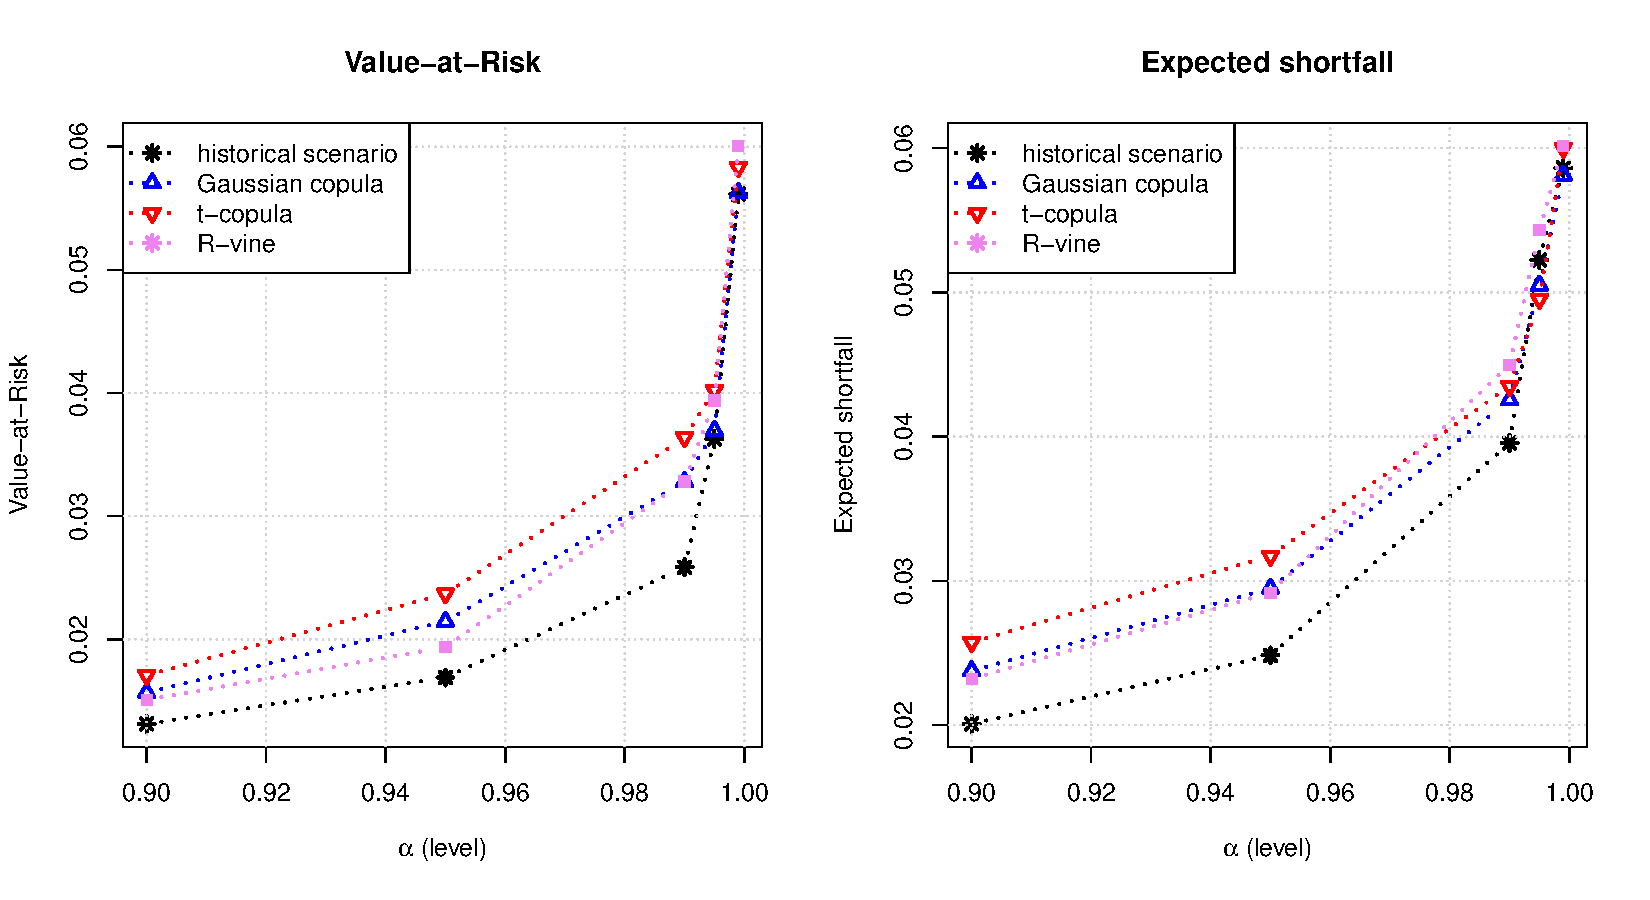
\includegraphics[height=0.6\paperheight]{VaR-ES.pdf}
        \caption{Точечные оценки риск-метрик VaR (слева) и CVaR (справа)}
    \end{figure}
\end{frame}

\subsection{Расчёт интервальных оценок риск-метрик}

\begin{frame}{\insertsection}
    \framesubtitle{\insertsubsection}
    \begin{table}
    \centering
    \caption{Характеристики для риск-метрики VaR, полученные с использованием бутстрап-процедуры для  Гауссовой\,/\,Стьюдента\,/\,R-vine копул}
    \label{tab:boot-var}
    \setlength{\tabcolsep}{5pt}
    \begin{adjustbox}{max width=\textwidth}
    \begin{tabular}{c*{4}{|r@{\,/\,}r@{\,/\,}r}} \toprule
    \multicolumn{1}{c|}{$\alpha$, \%} & \multicolumn{3}{c|}{$\overline{\textit{VaR}}_\alpha$, $\times 10^{-2}$} & \multicolumn{3}{c|}{$\Delta, \times 10^{-3}$} & \multicolumn{3}{c|}{SD, $\times 10^{-2}$} & \multicolumn{3}{c}{RMSE, $\times 10^{-3}$} \\ \midrule
    90.0   & $1.61$ & $1.62$ & $1.61$ & $2.99$ &  $3.03$ &  $2.96$ & $0.80$ & $0.79$ & $0.85$ & $3.10$ & $3.13$ & $3.08$ \\
    95.0   & $2.19$ & $2.20$ & $2.18$ & $5.00$ &  $5.06$ &  $4.93$ & $1.18$ & $1.37$ & $1.48$ & $5.14$ & $5.24$ & $5.14$ \\
    99.0   & $3.46$ & $3.50$ & $3.46$ & $8.71$ &  $9.11$ &  $8.78$ & $1.79$ & $2.32$ & $2.47$ & $8.89$ & $9.40$ & $9.11$ \\
    99.5 & $4.04$ & $4.21$ & $4.09$ & $4.15$ &  $5.82$ &  $4.64$ & $4.22$ & $6.10$ & $5.69$ & $5.91$ & $8.42$ & $7.33$ \\
    99.9 & $5.62$ & $5.53$ & $5.49$ & $0.05$ & $-0.86$ & $-1.21$ & $3.81$ & $5.18$ & $5.16$ & $3.81$ & $5.24$ & $5.29$ \\ \bottomrule
    \end{tabular}
    \end{adjustbox}
    \end{table}
\end{frame}

\begin{frame}{\insertsection}
    \framesubtitle{\insertsubsection}
    \begin{table}
    \centering
    \caption{Характеристики для риск-метрики СVaR, полученные с использованием бутстрап-процедуры для  Гауссовой\,/\,Стьюдента\,/\,R-vine копул}
    \label{tab:boot-es}
    \setlength{\tabcolsep}{5pt}
    \begin{adjustbox}{max width=\textwidth}
    \begin{tabular}{c*{4}{|r@{\,/\,}r@{\,/\,}r}} \toprule
    \multicolumn{1}{c|}{$\alpha$, \%} & \multicolumn{3}{c|}{$\overline{\textit{CVaR}}_\alpha$, $\times 10^{-2}$} & \multicolumn{3}{c|}{$\Delta, \times 10^{-3}$} & \multicolumn{3}{c|}{SD, $\times 10^{-2}$} & \multicolumn{3}{c}{RMSE, $\times 10^{-3}$} \\ \midrule
    90.0   & $2.46$ & $2.47$ & $2.45$ &  $4.53$ &  $4.62$ &  $4.43$ & $1.08$ & $1.32$ & $1.35$ & $4.66$ & $4.80$ & $4.63$ \\ 
    95.0   & $3.06$ & $3.08$ & $3.05$ &  $5.78$ &  $5.92$ &  $5.62$ & $1.49$ & $1.90$ & $1.91$ & $5.97$ & $6.21$ & $5.93$ \\ 
    99.0   & $4.36$ & $4.40$ & $4.34$ &  $4.08$ &  $4.46$ &  $3.86$ & $3.05$ & $4.31$ & $4.21$ & $5.09$ & $6.19$ & $5.71$ \\ 
    99.5 & $5.00$ & $4.99$ & $4.94$ & $-2.26$ & $-2.31$ & $-2.86$ & $4.05$ & $5.40$ & $5.34$ & $4.63$ & $5.87$ & $6.05$ \\ 
    99.9 & $5.76$ & $5.68$ & $5.68$ & $-1.03$ & $-1.79$ & $-1.88$ & $2.45$ & $3.86$ & $3.52$ & $2.65$ & $4.25$ & $3.98$ \\ \bottomrule
    \end{tabular}
    \end{adjustbox}
    \end{table}
\end{frame}

\begin{frame}{\insertsection}
    \framesubtitle{\insertsubsection}
    \begin{figure}
        \centering
        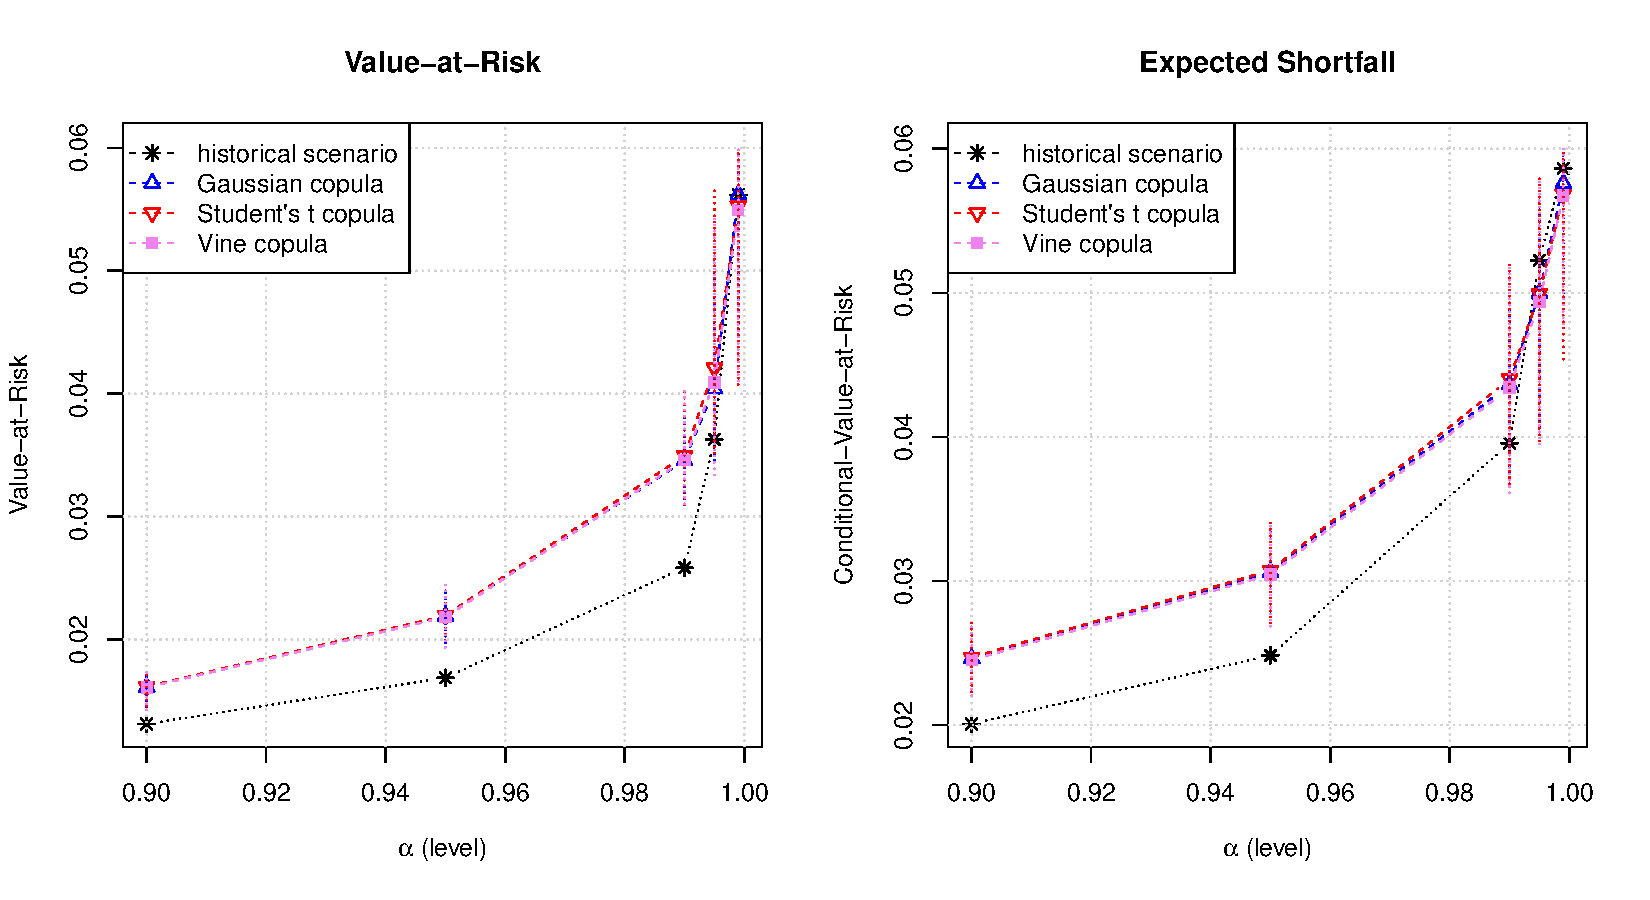
\includegraphics[height=0.6\paperheight]{VaR-ES-Bootstrap.pdf}
        \caption{Интервальные оценки риск-метрик VaR (слева) и CVaR (справа).\\Число итераций N = 200}
    \end{figure}
\end{frame}

\subsection{Моделирование кривых риск-метрик}

\begin{frame}{\insertsection}
    \framesubtitle{\insertsubsection}
    \begin{figure}
        \centering
        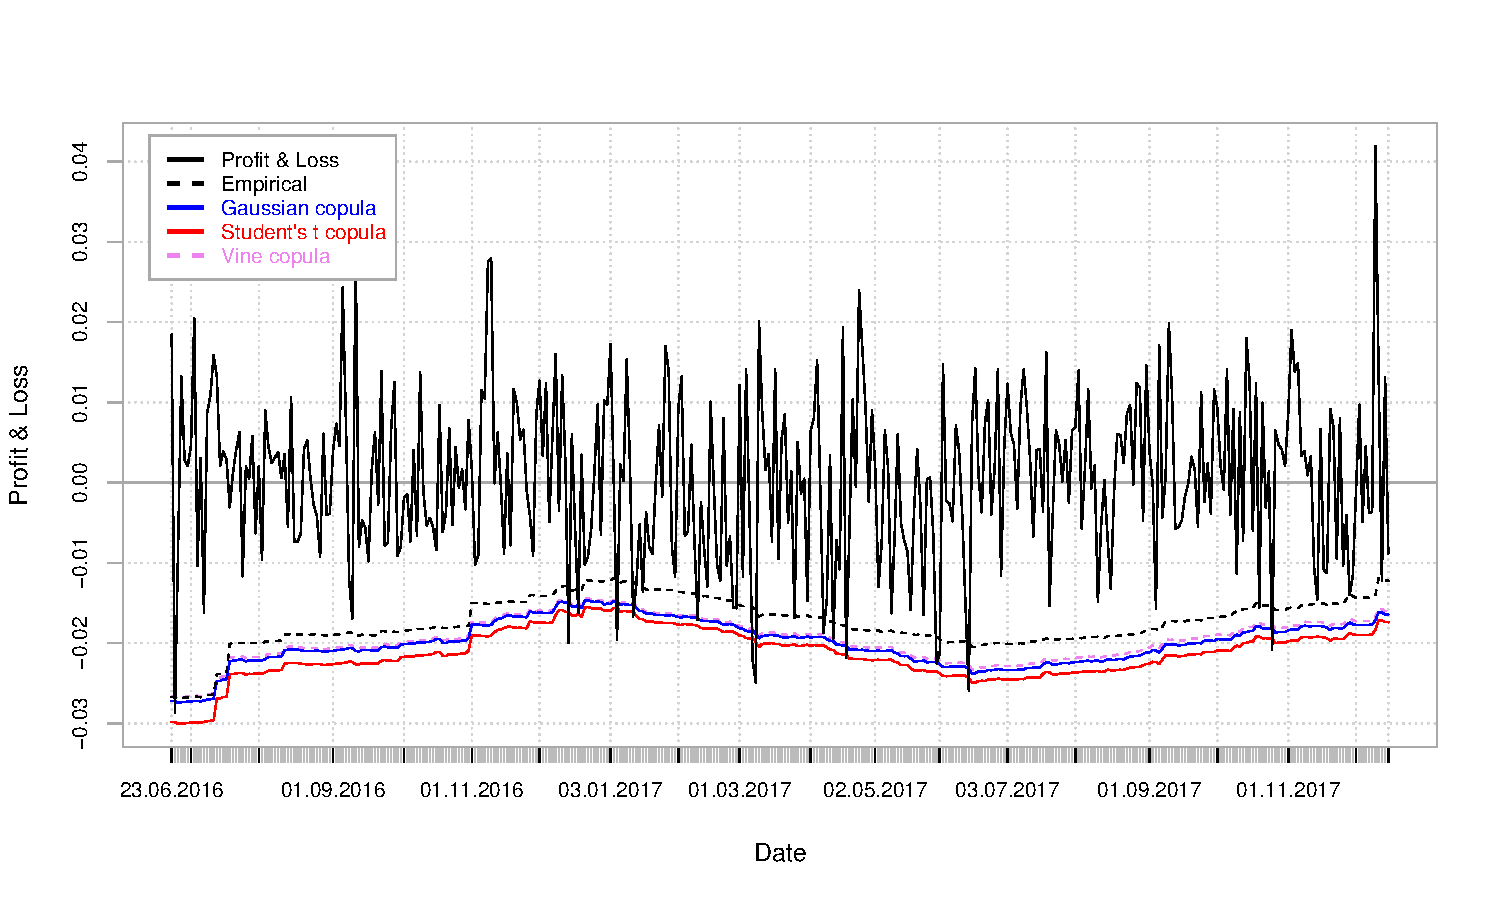
\includegraphics[height=0.6\paperheight]{VaRcurve.pdf}
        \caption{Смоделированные ряды VaR}
    \end{figure}
\end{frame}

\begin{frame}{\insertsection}
    \framesubtitle{\insertsubsection}
    \begin{figure}
        \centering
        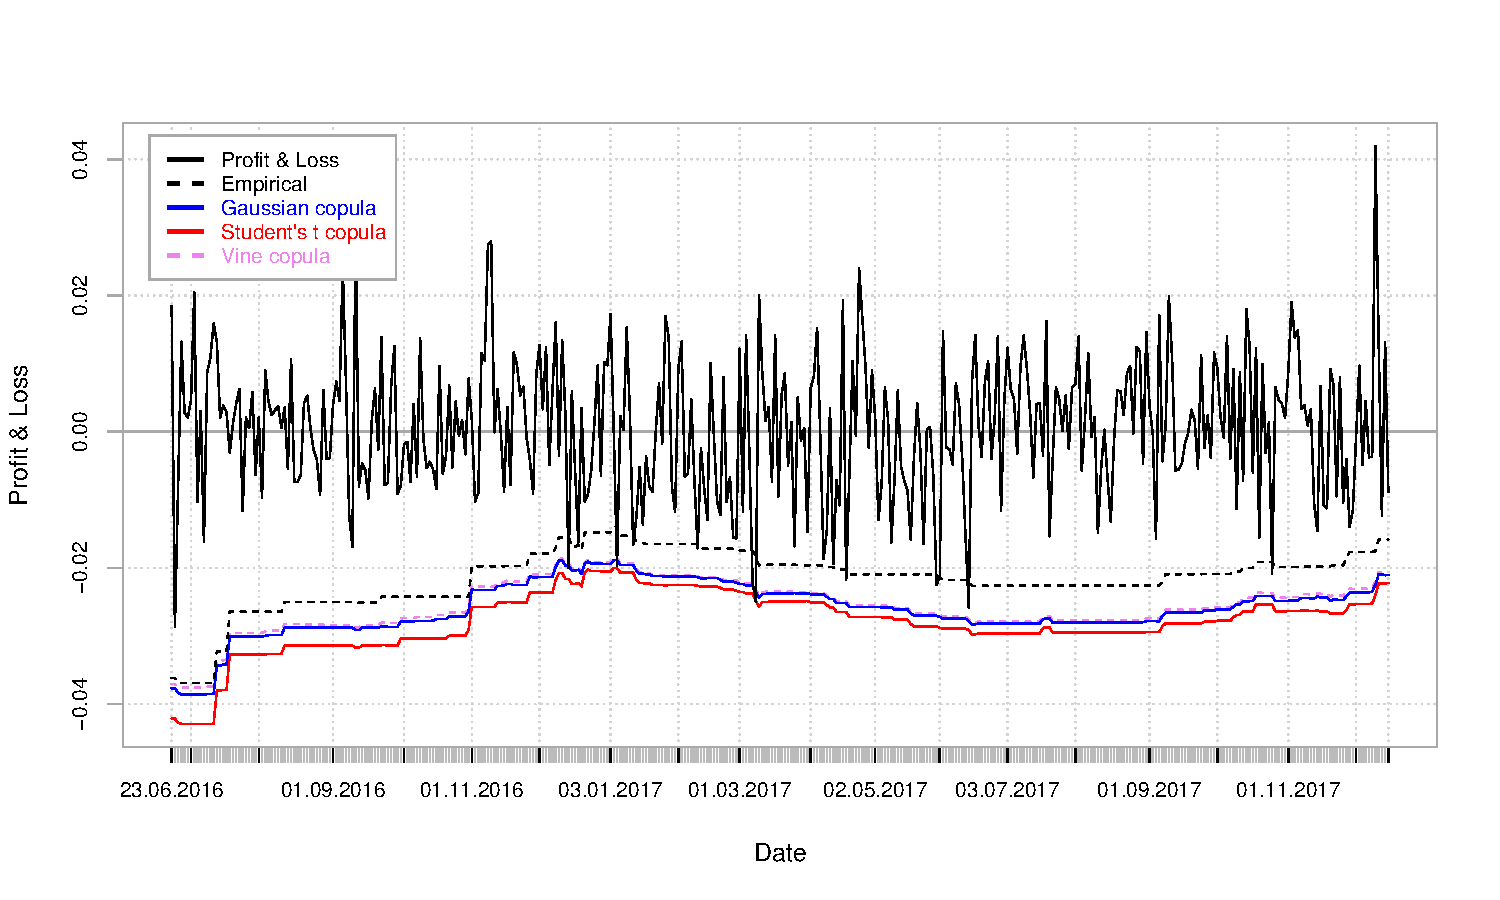
\includegraphics[height=0.6\paperheight]{EScurve.pdf}
        \caption{Смоделированные ряды CVaR}
    \end{figure}
\end{frame}

\begin{frame}{\insertsection}
    \framesubtitle{\insertsubsection}
    \begin{block}{Результаты теста Купича}
    \begin{table}
        \centering
        \caption{Значение статистики $LR$ и $p$-value теста Купича для кривых VaR на уровне 95\%}
        \label{tab:kupiec}
        \setlength{\tabcolsep}{10pt}
        \begin{tabular}{lrr} \toprule
            Метод & LR-статистика & $p$-value \\ \midrule
            эмпирический & 0.00 & 0.98 \\
            Гауссова копула & 3.02 & 0.08 \\
            $t$-копула & 10.29 & 0.00 \\
            R-vine & 2.17 & 0.14 \\ \bottomrule
        \end{tabular}
    \end{table}
    \end{block}
\end{frame}

\section{Заключение}

\begin{frame}{{}}
    \framesubtitle{\insertsection}
    \begin{block}{Нововведения}
        \begin{itemize}
            \item Применение копул к коротким временным рядам.
            \item Использование в связке с копулами маргинальных распределений, отличных от Гауссового.
            \item Использование вещественных чисел в качестве степеней свободы.
        \end{itemize}
    \end{block}
    \begin{block}{Выводы}
        \begin{itemize}
            \item Все используемые модели оказались консервативными на уровнях до 99\%.
            \item Наиболее адекватной оказалась модель R-иерархической копулы.
        \end{itemize}
    \end{block}
\end{frame}

\section{Список использованных источников}

% \begin{frame}{\insertsection}
    \bibliography{references.bib}
% \end{frame}

\end{document}